% =====================================================================
%  MAgent Battle-Zones -- homework description
%  Build:  make            (latexmk / pdflatex, two passes)
%     or:  tectonic main.tex
% =====================================================================
\documentclass[11pt,a4paper]{article}

\usepackage[utf8]{inputenc}
\usepackage[T1]{fontenc}
\usepackage{lmodern}
\usepackage{microtype}
\usepackage[margin=2.3cm]{geometry}
\usepackage{amsmath,amssymb}
\usepackage{graphicx}
\usepackage{booktabs}
\usepackage{tabularx}
\usepackage{enumitem}
\usepackage{xcolor}
\usepackage{float}
\usepackage{caption}
\usepackage{listings}
\usepackage{fancyhdr}
\usepackage[colorlinks=true,linkcolor=blue!50!black,urlcolor=blue!60!black,citecolor=blue!50!black]{hyperref}

% ---- edit these values for the course instance ----------------------
\newcommand{\CourseName}{Multi-Agent Reinforcement Learning}
\newcommand{\Semester}{Fall 2026}
\newcommand{\TeamSize}{2--3 students}
\newcommand{\Workload}{120--150}
\newcommand{\TimeZone}{ICT, UTC+7}
\newcommand{\DateStart}{Wed 18/11/2026}
\newcommand{\DateBaseA}{TBA (planned Wed 25/11/2026)}
\newcommand{\DateAEnd}{Tue 08/12/2026}
\newcommand{\DateBStart}{Wed 09/12/2026}
\newcommand{\DateBEnd}{Sat 12/12/2026}
\newcommand{\DateEnd}{Wed 16/12/2026}
\newcommand{\DateInterview}{after 16/12/2026}


\pagestyle{fancy}
\fancyhf{}
\lhead{\small \CourseName}
\rhead{\small MAgent Battle-Zones homework}
\cfoot{\small \thepage}

\lstset{basicstyle=\ttfamily\small, columns=fullflexible, breaklines=true,
        frame=single, rulecolor=\color{black!25}, backgroundcolor=\color{black!3},
        keywordstyle=\color{blue!60!black}, commentstyle=\color{black!55},
        language=Python, showstringspaces=false}

\setlist{itemsep=2pt, topsep=4pt}
\newcommand{\red}[1]{\textcolor{red!70!black}{#1}}
\newcommand{\green}[1]{\textcolor{green!45!black}{#1}}
\newcommand{\code}[1]{\texttt{#1}}

\title{\textbf{MAgent Battle-Zones}\\[2pt]
       \large Multi-Agent Reinforcement Learning Homework}
\author{\CourseName\ --- \Semester}
\date{Released \DateStart\quad$\cdot$\quad Final deadline \DateEnd}

\begin{document}
\maketitle
\thispagestyle{fancy}

\begin{abstract}
\noindent Two armies of 81 agents fight on a $45\times45$ grid.  The battlefield
contains \red{red squares}, where wounded agents cannot recover, and
\green{green squares}, where they recover twice as fast.  In the \emph{easy} setting the
layout of the squares is fixed; in the \emph{hard} setting it is drawn at random at every
episode.  You will implement, train and compare cooperative multi-agent reinforcement
learning (MARL) algorithms---at least one \emph{value-based} and one
\emph{policy-based}---under a strict compute budget (60 minutes of Kaggle GPU per
notebook), and finally confront your agents with well-trained baselines.  The expected
workload is \textbf{\Workload\ hours per student}.
\end{abstract}

\tableofcontents

% ---------------------------------------------------------------------
\section{Overview}
% ---------------------------------------------------------------------

\paragraph{Learning goals.}
After this homework you should be able to
\begin{enumerate}
  \item formalise a large-scale cooperative/competitive game as a (partially observable)
        stochastic game and choose a suitable training paradigm (independent learning vs.\
        centralised training with decentralised execution, CTDE);
  \item implement and debug a value-decomposition method (VDN, QMIX, \dots) and a
        multi-agent policy-gradient method (MAPPO, HAPPO, MADDPG, \dots);
  \item study generalisation: a policy trained on one map vs.\ a distribution of maps;
  \item run honest, reproducible experiments under a fixed compute budget and report them.
\end{enumerate}

\paragraph{Organisation.}
The homework is done in teams of \TeamSize\ and has two phases
(Table~\ref{tab:timeline}):
\begin{itemize}
  \item \textbf{Subtask A} (\DateStart\ -- \DateAEnd): algorithms, training and evaluation in
        both settings; submission of two notebooks (code freeze).
  \item \textbf{Subtask B} (\DateBStart\ -- \DateBEnd): your \emph{frozen} notebooks are run
        against several well-trained baselines in the hard setting.
\end{itemize}
The report is due on \DateEnd; interviews follow.

\begin{table}[H]
\centering
\caption{Timeline (all deadlines 23:59, \TimeZone).}
\label{tab:timeline}
\begin{tabularx}{\linewidth}{@{}l l X@{}}
\toprule
\textbf{Date} & \textbf{Event} & \textbf{Details} \\
\midrule
\DateStart & Release & Task description, \code{battle\_zones} environment, starting-kit notebook. \\
\DateBaseA & Base policy (hard) & First baseline policy for the hard setting (Subtask A opponent). \\
\DateAEnd & \textbf{Subtask A deadline} & Two notebooks + exported policies + \code{results\_A.json}. \textbf{Code freeze.} \\
\DateBStart & Subtask B starts & Evaluation baselines released (one week before the final deadline). \\
\DateBEnd & \textbf{Subtask B deadline} & Executed notebooks + \code{results\_B.json}. Only running code is allowed. \\
\DateEnd & \textbf{Final deadline} & Report (PDF). \\
\DateInterview & Interviews & Schedule announced on the course page. \\
\bottomrule
\end{tabularx}
\end{table}

% ---------------------------------------------------------------------
\section{The Battle-Zones environment}
% ---------------------------------------------------------------------

Battle-Zones extends the \code{battle} environment of MAgent2~\cite{magent,magent2}
(\url{https://magent2.farama.org/environments/battle/}).  It is distributed as the Python
package \code{battle\_zones}, which ships a minimally patched copy of the MAgent2 C++ engine
(one new per-cell HP-regeneration map) and is used through the PettingZoo
\emph{Parallel} API~\cite{pettingzoo}:

\begin{lstlisting}
import battle_zones as bz
env = bz.parallel_env("hard")          # or "easy";  max_cycles=500 by default
obs, infos = env.reset(seed=0)         # dict: agent name -> (13, 13, 7) array
while env.agents:
    actions = {a: policy(obs[a]) for a in env.agents}
    obs, rewards, terminations, truncations, infos = env.step(actions)
print(env.get_stats())                 # alive counts, kills, deaths, winner
\end{lstlisting}

\subsection{Unchanged from MAgent2 \code{battle}}

\begin{itemize}
  \item \textbf{Map}: $45\times45$ cells, the outer ring is wall (playable cells
        $1,\dots,43$).
  \item \textbf{Agents}: two teams, \code{red\_0..red\_80} (left) and
        \code{blue\_0..blue\_80} (right), each a $9\times9$ block.  Agents have 10 HP,
        speed 2, view radius 6, attack radius 1.5; one attack removes 2 HP.  An agent
        dies when its HP drops below 0.
  \item \textbf{Actions}: \code{Discrete(21)}: 13 moves on the disc of radius 2 (action
        6 = stay) and 8 attacks on the neighbouring cells.  Attacks on team mates are
        ignored.
  \item \textbf{Rewards} (per agent, summed when several apply): $+5$ for killing an
        opponent, $-0.005$ per step, $-0.1$ per attack, $+0.2$ per attack that hits an
        opponent, $-0.1$ for dying.
\end{itemize}

\subsection{What is new}

\paragraph{Zones.}
Every cell has an HP-regeneration multiplier $\mu(x,y)$; an alive agent standing on
$(x,y)$ recovers $0.1\,\mu(x,y)$ HP per step (capped at 10 HP):

\begin{table}[H]
\centering
\begin{tabular}{@{}lcc@{}}
\toprule
Cell type & $\mu$ & HP recovered per step \\
\midrule
normal & 1 & 0.1 \\
\red{red square} & 0 & 0 \\
\green{green square} & 2 & 0.2 \\
\bottomrule
\end{tabular}
\end{table}
\noindent Where a red and a green square overlap, red wins.  Zones do not block movement
and do not change rewards: their effect on the game is only through HP.

\paragraph{Observation} (per agent, $13\times13\times7$, layout \code{[row=y, col=x, c]},
cells outside the view disc are 0):
\code{[obstacle, my\_team, my\_team\_hp, enemy, enemy\_hp, red\_zone, green\_zone]}.
HP values are normalised to $[0,1]$.  Figure~\ref{fig:obs} shows an example.

\begin{figure}[H]
\centering
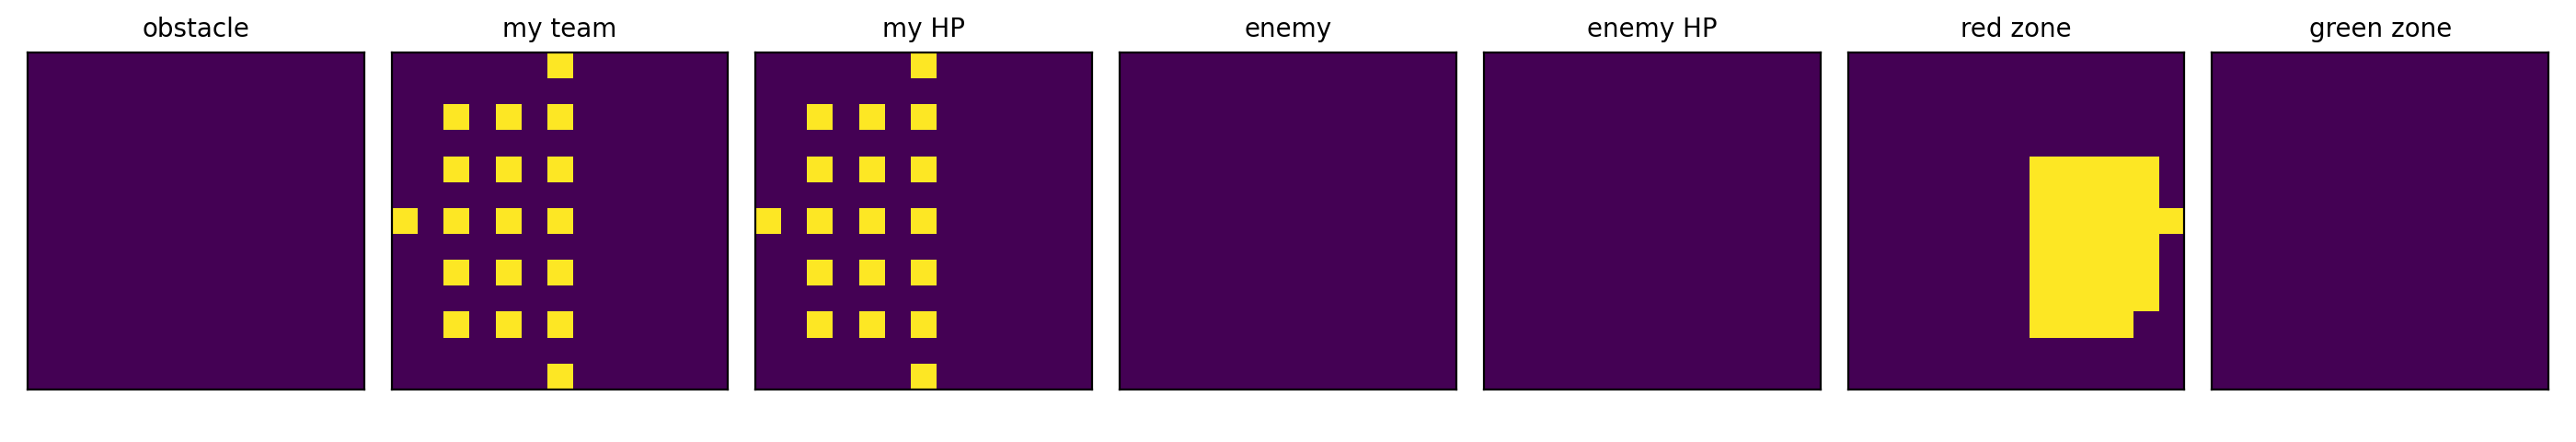
\includegraphics[width=\linewidth]{figures/obs_channels.png}
\caption{The 7 observation channels of a red front-line agent at reset (easy setting): the
red square in the middle of the battlefield is already visible.}
\label{fig:obs}
\end{figure}

\paragraph{Global state} (\code{env.state()}, $45\times45\times7$, layout \code{[y, x, c]}):
\code{[obstacle, red, red\_hp, blue, blue\_hp, red\_zone, green\_zone]}.  It may be used
\emph{during training only} (centralised critics, mixing networks).
\code{env.state(team="blue")} returns the blue-centric version (own team first, mirrored).

\paragraph{Symmetry and mirrored blue team.}
Armies and zone layouts are mirror-symmetric with respect to the vertical centre line, so
neither side is advantaged.  The observations of blue agents are flipped horizontally and
their actions are flipped back by the environment: \emph{every agent perceives the world as
if its army started on the left}.  Hence a single policy can control either team, which is
what makes self-play and Subtask B possible.

\paragraph{End of an episode and winner.}
An episode ends when one army is eliminated or after \code{max\_cycles}$\,=500$ steps.
The team with more surviving agents wins; equal numbers give a draw.

\subsection{The two settings}

\paragraph{(a) Easy -- fixed map.}
The same layout is used for training and evaluation (Figure~\ref{fig:easy}): one $7\times7$
red square in the no-man's-land between the armies (cells $x,y\in[19,25]$) and four
$5\times5$ green squares on the flanks behind the armies (top-left corners $(9,4)$,
$(31,4)$, $(9,36)$, $(31,36)$).

\begin{figure}[H]
\centering
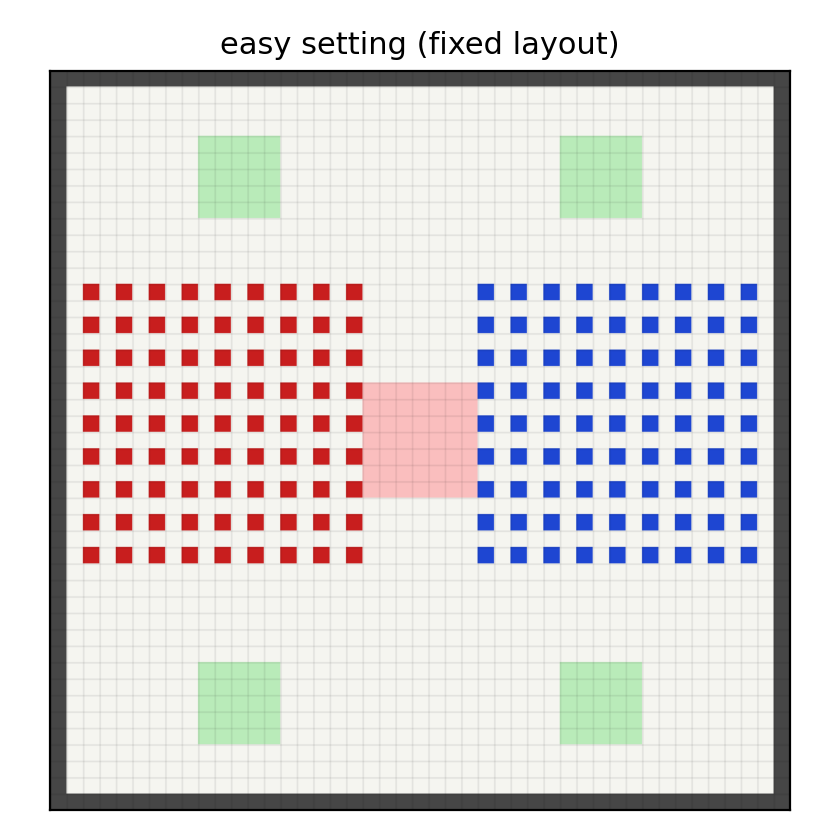
\includegraphics[width=0.42\linewidth]{figures/easy_map.png}
\caption{Easy setting.  Red/blue dots: agents (faded = wounded).  Pink: red squares.
Light green: green squares.}
\label{fig:easy}
\end{figure}

\paragraph{(b) Hard -- random maps.}
At every \code{reset} a new layout is drawn independently and uniformly:
\begin{align*}
  n_{\text{red}} &\sim \mathcal{U}\{1,2,3\}, \qquad
  n_{\text{green}} \sim \mathcal{U}\{1,2,3\},\\
  s_k &\sim \mathcal{U}\{3,\dots,9\} \quad\text{(side of square $k$)},\\
  x_k &\sim \mathcal{U}\{1,\dots,\min(22,\,44-s_k)\},\qquad
  y_k \sim \mathcal{U}\{1,\dots,44-s_k\}\quad\text{(top-left corner)},
\end{align*}
and every square is completed by its mirror image $x \mapsto 44-x$, which keeps the map
fair.  A map therefore contains 2--6 red and 2--6 green squares (fewer if mirrors
coincide).  Evaluation uses fixed seeds so that every team meets the same maps.
The distribution is \code{bz.HardZoneDistribution()}; do not change it for evaluation.

\begin{figure}[H]
\centering
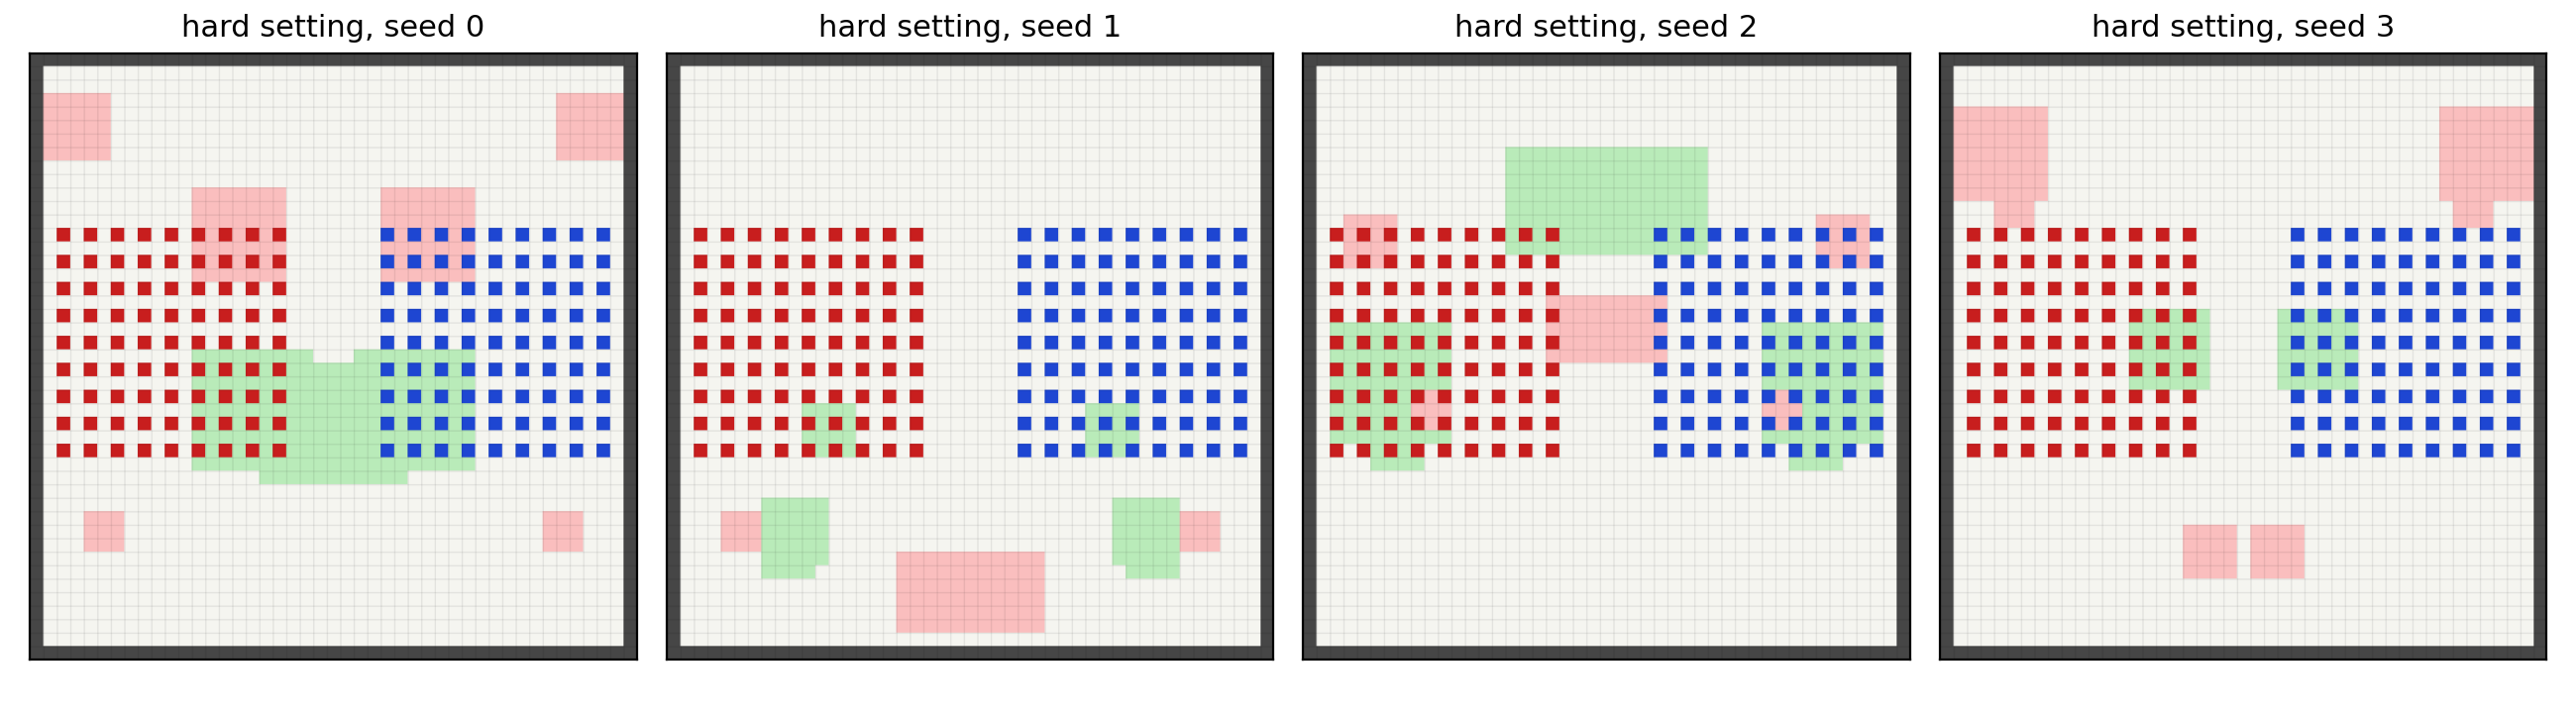
\includegraphics[width=\linewidth]{figures/hard_maps.png}
\caption{Four maps drawn from the hard-setting distribution.}
\label{fig:hard}
\end{figure}

% ---------------------------------------------------------------------
\section{Starting kit}
% ---------------------------------------------------------------------

The notebook \code{starter\_kit.ipynb} runs on Kaggle (GPU accelerator, internet on).  It
\begin{enumerate}[label=(\alph*)]
  \item installs MAgent2 (\code{pip install magent2==0.3.4});
  \item installs the \code{battle\_zones} environment (course dataset or repository; the
        engine is compiled automatically in $\approx$10\,s);
  \item runs the easy and the hard configuration and visualises the maps;
  \item trains a simple \textbf{IPPO} agent~\cite{ippo} (red) against a \textbf{random}
        policy (blue) following the CTDE paradigm: shared actor-critic parameters,
        centralised training on the pooled experience of the 81 agents, decentralised
        execution from local $13\times13$ observations only; 10 minutes per setting;
  \item reports the score: win/draw/loss rates, kill\,\% and death\,\%, K/D ratio, and
        saves a replay GIF.
\end{enumerate}

\paragraph{Policy interface.}
A trained policy is exported as a \textbf{TorchScript} module mapping a batch of
observations \code{(N,13,13,7)} (float32) to action logits \code{(N,21)}.  The baselines
are distributed in the same format and are loaded with \code{load\_policy(path)}.  Any
object with a method \code{act(obs)} returning one integer action per row of \code{obs}
can be evaluated with the kit's function
\code{evaluate(red\_policy, blue\_policy, setting, n\_episodes)}.
Your policies \emph{must} be exportable in this format (decentralised execution: one agent,
one local observation; recurrent policies must keep their state inside the module and
document it).

\paragraph{Metrics.}
For $E$ evaluation episodes with army size $n=81$:
\begin{gather*}
  \text{win}=\tfrac{1}{E}\#\{\text{episodes won}\},\qquad
  \text{draw}=\tfrac{1}{E}\#\{\text{draws}\},\qquad
  \text{loss}=1-\text{win}-\text{draw},\\
  \text{kill\,\%}=100\,\frac{\sum_e \text{kills}_e}{nE},\qquad
  \text{death\,\%}=100\,\frac{\sum_e \text{deaths}_e}{nE},\qquad
  \text{K/D}=\frac{\sum_e \text{kills}_e}{\max(1,\sum_e \text{deaths}_e)} .
\end{gather*}

% ---------------------------------------------------------------------
\section{Subtask A -- algorithms}
\emph{Period: \DateStart\ -- \DateAEnd.}\par\smallskip
% ---------------------------------------------------------------------

A \textbf{base policy} for the hard setting is provided (\DateBaseA).  Implement and train
\textbf{at least two} MARL algorithms:
\begin{enumerate}
  \item a \textbf{value-based} method: VDN~\cite{vdn}, QMIX~\cite{qmix}, QTRAN, QPLEX, \dots;
  \item a \textbf{policy-based} method: MAPPO~\cite{mappo}, HAPPO~\cite{happo},
        MADDPG~\cite{maddpg}, COMA, \dots
\end{enumerate}
Each algorithm is delivered as \textbf{one self-contained Kaggle notebook} that installs the
environment, trains and evaluates in \textbf{both} settings:

\begin{table}[H]
\centering
\begin{tabular}{@{}llll@{}}
\toprule
Train on & Evaluate on & Opponents & Episodes \\
\midrule
easy & easy & random, base policy & 20 each \\
hard & hard & random, base policy & 50 each \\
easy & hard & random, base policy & 50 each (transfer) \\
\bottomrule
\end{tabular}
\end{table}

\noindent Use the evaluation function and the seeds of the starting kit.

\paragraph{Rules.}
\begin{itemize}
  \item \textbf{Compute budget}: the total training time of one notebook (both settings
        together) is at most \textbf{60 minutes on a Kaggle GPU}; evaluation time is not
        counted.  Enforce it with a wall-clock check in the code, as the kit does.
  \item You may change the network, the rewards used for learning (reward shaping), the
        opponent(s) used during training (random, base policy, self-play, league\dots),
        curricula and hyper-parameters.  You may \emph{not} modify the environment
        dynamics, the observation given to the executed policy, or the evaluation code.
  \item No pre-trained weights from outside the notebook, except the provided base policy
        (as an opponent or for initialisation---say so in the report).
  \item Running the notebook from top to bottom on Kaggle must reproduce your results
        (fix and report the seeds).
\end{itemize}

\paragraph{Deliverables} (by \DateAEnd, after which the notebooks are \textbf{frozen}):
\begin{itemize}
  \item \code{A\_value\_based.ipynb} and \code{A\_policy\_based.ipynb}, executed, with outputs;
  \item the exported policies \code{<algo>\_easy.pt} and \code{<algo>\_hard.pt};
  \item \code{results\_A.json} (all metrics of the table above);
  \item the name of the policy you nominate for Subtask B.
\end{itemize}

% ---------------------------------------------------------------------
\section{Subtask B -- against the baselines}
\emph{Period: \DateBStart\ -- \DateBEnd.}\par\smallskip
% ---------------------------------------------------------------------

On \DateBStart\ several well-trained baselines for the \textbf{hard} setting are released
(TorchScript, same interface).  Each team evaluates its nominated policy against every
baseline: \textbf{50 episodes per baseline}, hard setting, official seeds, your policy
plays red, the baseline plays blue.

\paragraph{Only running code is allowed.}
The notebooks submitted on \DateAEnd\ are fixed.  During Subtask B you may only change the
paths of the baseline files and of your exported policy in the configuration cell, and run
the evaluation.  No retraining, fine-tuning or code change; submitted notebooks are
compared with the frozen version.  The staff re-runs the evaluation to check the numbers.

\paragraph{Deliverables} (by \DateBEnd): the executed evaluation notebook and
\code{results\_B.json}.

\paragraph{Score.}
For baseline $b$ let $W_b, D_b$ be the win and draw rates and $k_b, d_b$ the kill and
death percentages.  The Subtask B score is
\[
  S_B \;=\; \frac{1}{|\mathcal{B}|}\sum_{b\in\mathcal{B}}
  \Big[\,0.8\,(W_b + 0.5\,D_b) \;+\; 0.2\,\frac{k_b - d_b + 100}{200}\Big] \in [0,1],
\]
and part 3 of the grade is $25 \cdot S_B$ points (the staff may rescale linearly if the
baselines turn out to be too strong for every team).

% ---------------------------------------------------------------------
\section{Evaluation}
% ---------------------------------------------------------------------

\begin{table}[H]
\centering
\begin{tabularx}{\linewidth}{@{}l c X@{}}
\toprule
\textbf{Part} & \textbf{Weight} & \textbf{Criteria} \\
\midrule
1. Report & 25\% & Clear problem formulation; description of the algorithms and of the
CTDE design choices; experimental protocol; results for every row of the Subtask A table
(with variability over seeds where affordable); training curves; ablations (e.g.\ zone
channels, reward shaping, opponent choice); analysis of easy vs.\ hard and of the transfer;
discussion of Subtask B; honest limitations. \\
2. Code base & 25\% & Correct implementation of both algorithm families; runs on Kaggle
end-to-end within budget; reproducibility (seeds, logged hyper-parameters); readability and
structure; exported policies respect the interface. \\
3. Subtask B result & 25\% & $25\cdot S_B$, see Section 5. \\
4. Interview & 25\% & Individual: every member explains the code, the algorithms and the
results; answers questions on MARL theory used in the homework.  Grades may differ between
team members. \\
\bottomrule
\end{tabularx}
\end{table}

\paragraph{Report format.}
PDF, at most \textbf{8 pages} (references and appendix excluded), names and student IDs on
the first page, a contribution statement (who did what), and links to the Kaggle notebooks.

\paragraph{Academic integrity.}
You may use public implementations (e.g.\ EPyMARL, MAPPO, HARL) as references, but the
code you submit must be written or substantially adapted by your team and every source
must be cited.  Use of AI assistants must be declared in the report.  Sharing code or
trained policies between teams is forbidden.

\paragraph{Suggested workload} (per student, \Workload\ h in total):
reading and environment study 15\,h; value-based method 35--45\,h; policy-based method
35--45\,h; experiments and ablations 20\,h; Subtask B 5\,h; report 15\,h; interview
preparation 5\,h.

% ---------------------------------------------------------------------
\section{Practical notes}
% ---------------------------------------------------------------------
\begin{itemize}
  \item With 81 agents, a single environment step yields 81 transitions: parameter sharing
        is a strong default.  The kit reaches
        $\approx$200 environment steps/s on one CPU core; parallel environments (one
        process each) help a lot on Kaggle's 4 cores.
  \item Dead agents leave the PettingZoo dict; keep a fixed slot per agent and an alive mask
        (see \code{stack\_obs} in the kit).
  \item For value decomposition the number of alive agents changes over time: mask dead
        agents in the mixer.  For MAPPO, the global state $45\times45\times7$ is a natural
        critic input.
  \item \textbf{Reward pitfalls.}  With the stock rewards ($-0.005$ per step, only $-0.1$ for
        dying) an agent that cannot kill learns to die early (it is cheaper than surviving
        500 steps); without the step penalty it learns to idle.  The kit trains with
        \code{step\_reward=0}, \code{dead\_penalty=-1}, \code{attack\_penalty=-0.02} and a
        potential-based shaping term $c\,(\gamma\,\phi(o')-\phi(o))$, $\phi(o)$ = number of
        visible enemies~\cite{shaping}; with it, IPPO beats the random policy within a few
        minutes.  Beating trained opponents is a different story.
  \item Zones matter mostly for long fights: retreating to a green square to heal or
        luring the enemy onto a red square are behaviours you may observe and analyse.
\end{itemize}

\begin{thebibliography}{99}\small
\bibitem{magent} L.~Zheng et al. \emph{MAgent: A many-agent reinforcement learning platform
for artificial collective intelligence.} AAAI 2018.
\bibitem{magent2} Farama Foundation. \emph{MAgent2}. \url{https://magent2.farama.org}.
\bibitem{pettingzoo} J.~K.~Terry et al. \emph{PettingZoo: Gym for multi-agent reinforcement
learning.} NeurIPS 2021.
\bibitem{ippo} C.~Schroeder de Witt et al. \emph{Is independent learning all you need in the
StarCraft multi-agent challenge?} arXiv:2011.09533, 2020.
\bibitem{vdn} P.~Sunehag et al. \emph{Value-decomposition networks for cooperative
multi-agent learning.} AAMAS 2018.
\bibitem{qmix} T.~Rashid et al. \emph{QMIX: Monotonic value function factorisation for deep
multi-agent reinforcement learning.} ICML 2018.
\bibitem{mappo} C.~Yu et al. \emph{The surprising effectiveness of PPO in cooperative
multi-agent games.} NeurIPS 2022.
\bibitem{happo} J.~G.~Kuba et al. \emph{Trust region policy optimisation in multi-agent
reinforcement learning.} ICLR 2022.
\bibitem{shaping} A.~Y.~Ng, D.~Harada, S.~Russell. \emph{Policy invariance under reward
transformations: theory and application to reward shaping.} ICML 1999.
\bibitem{maddpg} R.~Lowe et al. \emph{Multi-agent actor-critic for mixed
cooperative-competitive environments.} NeurIPS 2017.
\end{thebibliography}

\end{document}
